\documentclass[12pt,a4paper,oneside]{article}
\usepackage{amsmath,amsthm,amsfonts,amssymb}
\usepackage{pst-eucl,pstricks,pstricks-add}
\usepackage[utf8]{inputenc}
%\usepackage[latin1]{inputenc}
\usepackage[spanish,activeacute]{babel}
\usepackage[a4paper,margin=2.5cm]{geometry}
\usepackage{times}
\usepackage[T1]{fontenc}
\usepackage{titlesec}
\usepackage{color}
\usepackage{url}
\usepackage{float}
\usepackage{cite}
\usepackage{graphicx}
\usepackage{multicol}
\usepackage{lipsum}
\usepackage{transparent}
\usepackage{eso-pic}
%\AddToShipoutPicture*{
   % \put(0,0){
        %\parbox[b][\paperheight]{\paperwidth}{%
           % \vfill
            %\centering
            %{\transparent{0.5}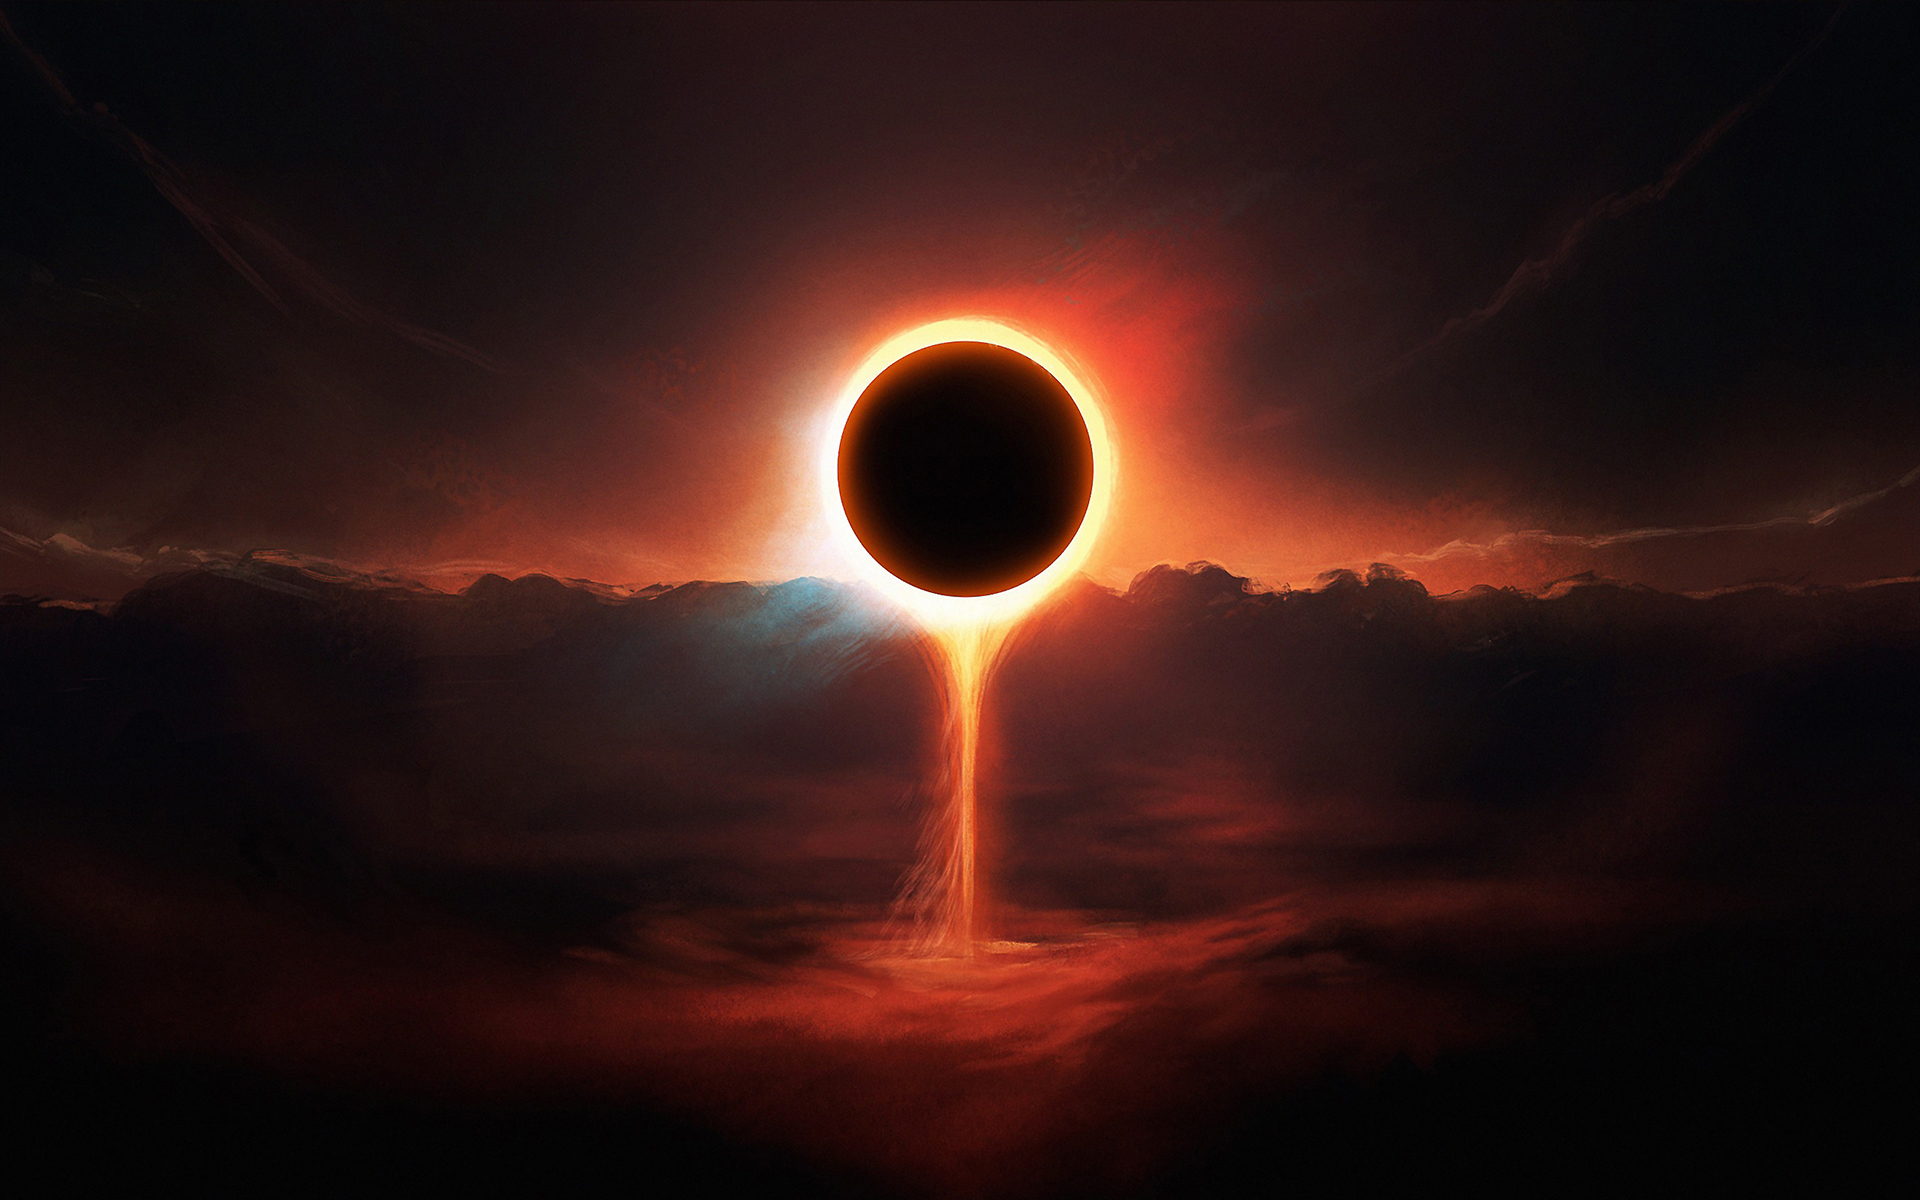
\includegraphics[width=3.5\textwidth]{febrero}}%
           % \vfill
       % }
   % }
%}
%\AddToShipoutPicture*{
   % \put(0,0){
      %  \parbox[b][\paperheight]{\paperwidth}{%
           % \vfill
           % \centering
           % {\transparent{0.5}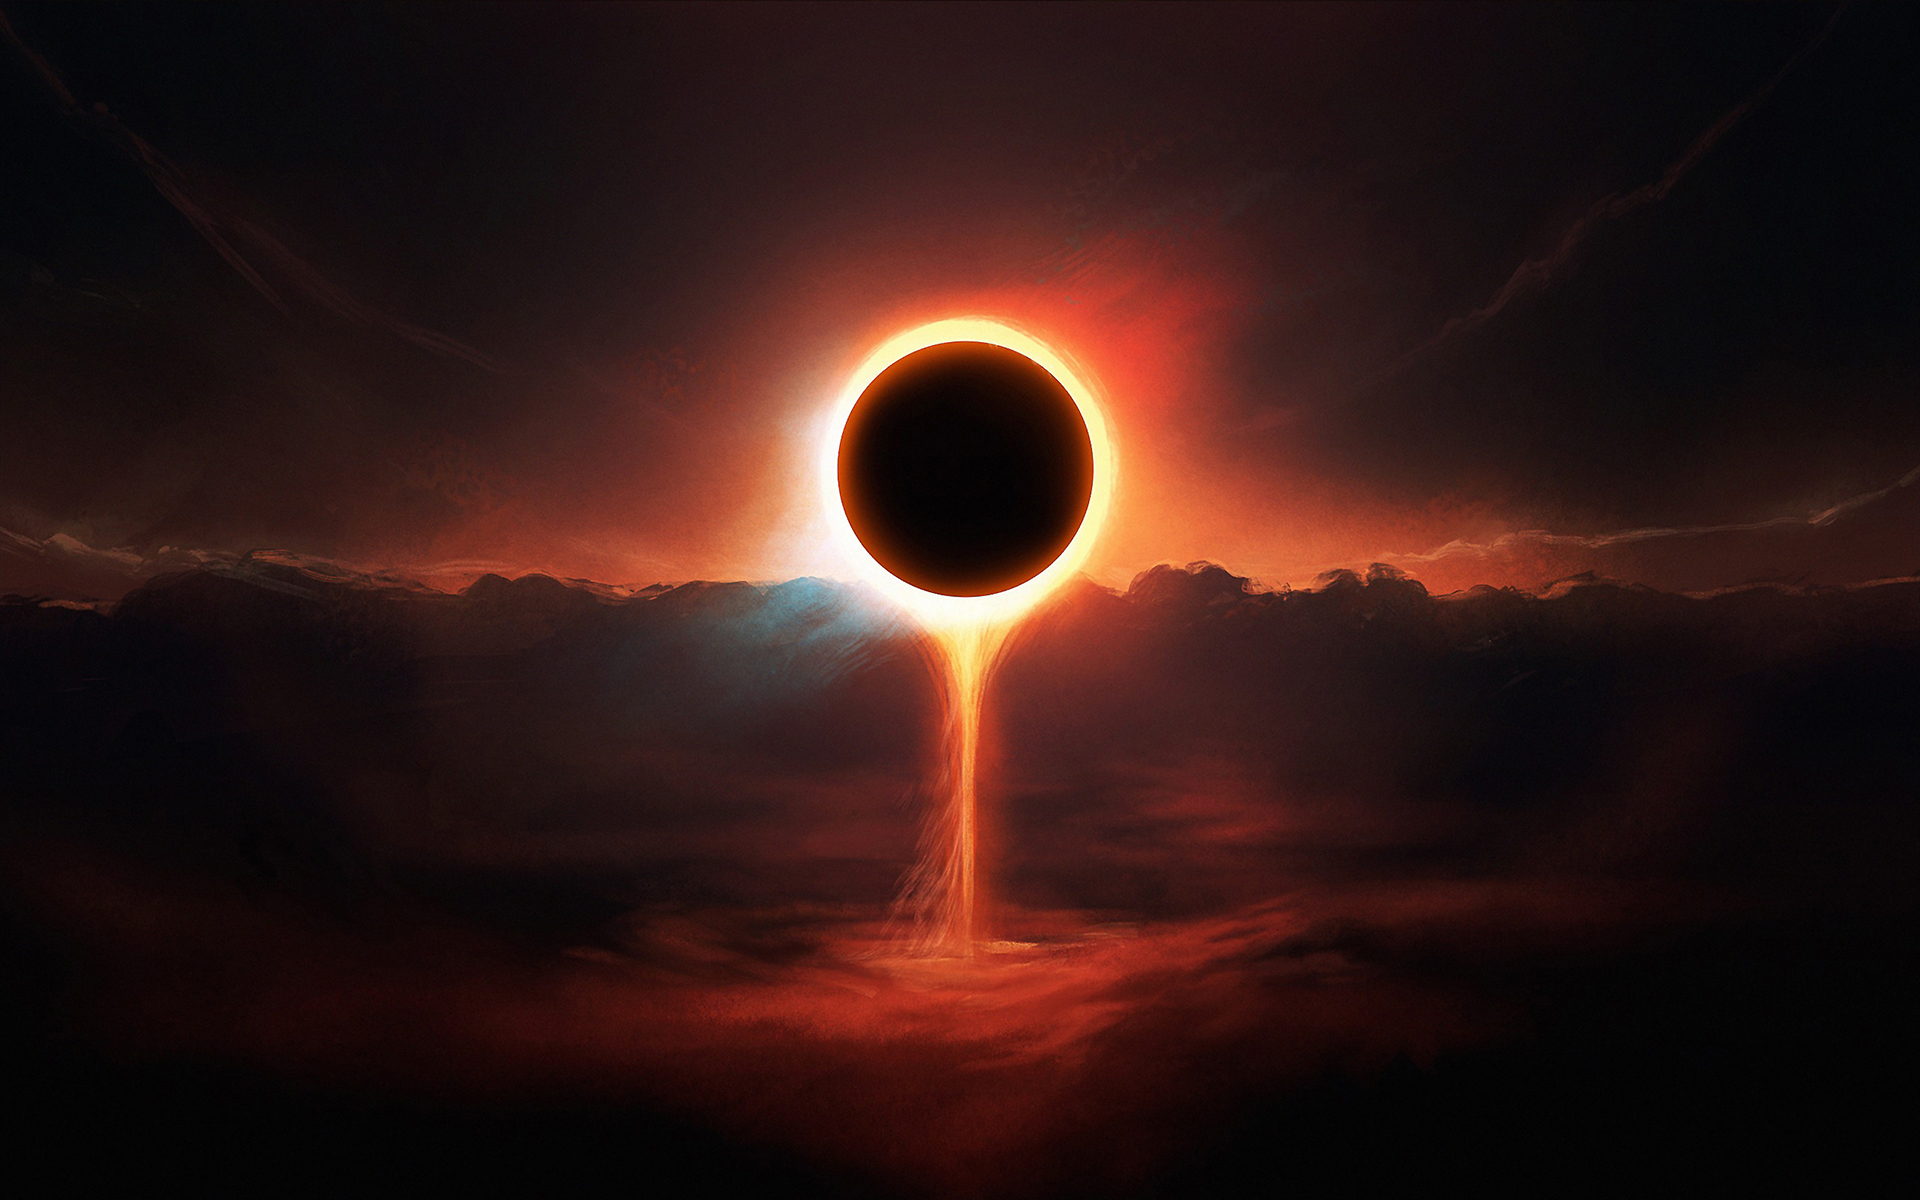
\includegraphics[width=3\textwidth]{febrero}}%
          %  \vfill
       % }
    %}
%}

\usepackage{draftwatermark}
\SetWatermarkText{\transparent{0.4}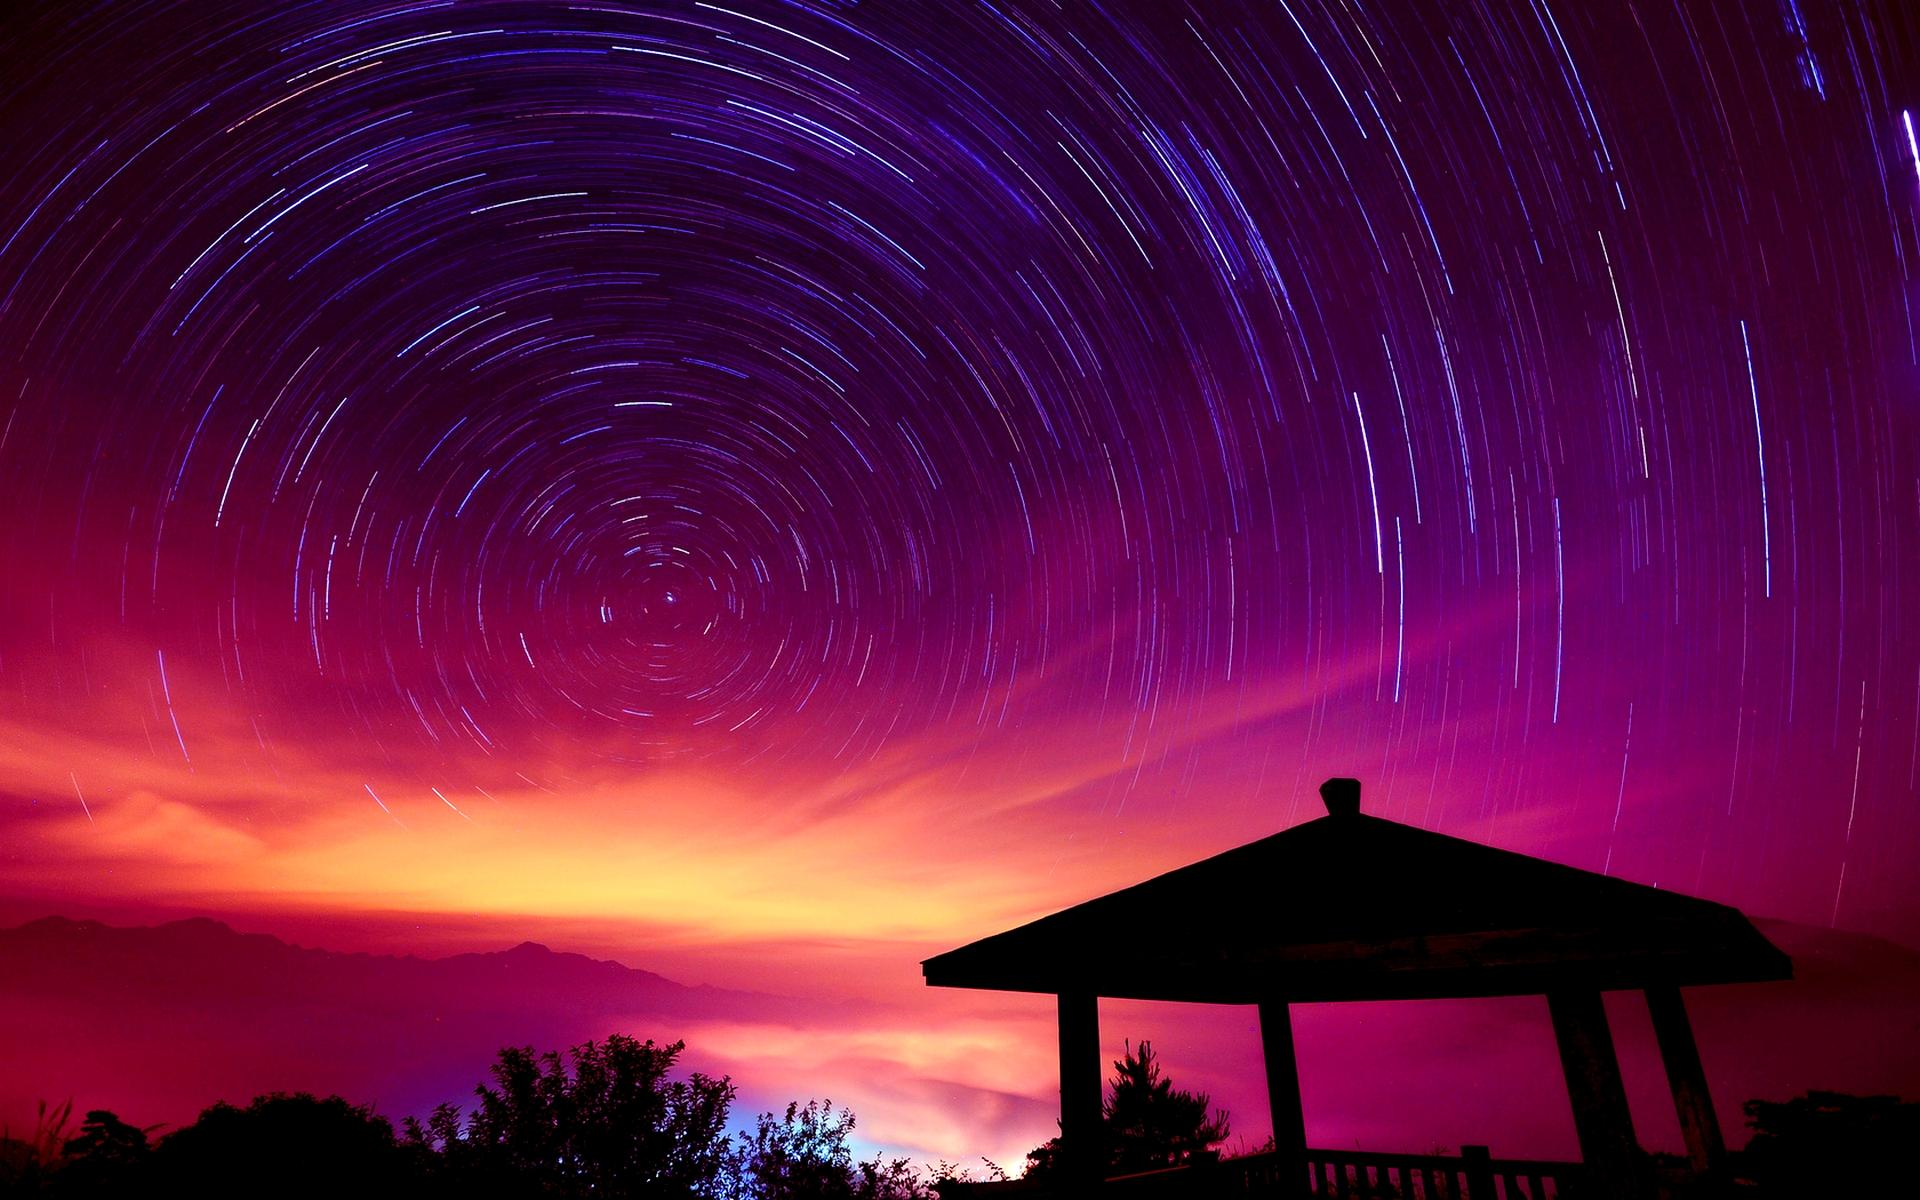
\includegraphics[scale=0.9,trim={5cm 0 5cm 0},clip,angle=-45]{lluvia}}
\usepackage{gensymb}
\usepackage{hyperref}
\usepackage{setspace}%\doublespace %para doble espacio
\onehalfspace %para espacio y medio
\newcommand{\code}[1]{\fcolorbox{blue!80}{gray!10}{#1}}
\parindent=0mm
\begin{document}
%\SweaveOpts{concordance=TRUE}
\rule[1mm]{170mm}{0.20mm}
\begin{minipage}[d]{30mm}
\begin{center}

\includegraphics[scale=0.30]{logo_epn.png}
\end{center}
\end{minipage}
\begin{minipage}[d]{100mm}
\begin{center}
\vspace{0.5cm}
\textsf{\textbf{\large ESCUELA POLITÉCNICA NACIONAL}}\\
\textsf{\textbf{\small OBSERVATORIO ASTRONÓMICO DE QUITO}}\\
\end{center}
\end{minipage}
\begin{minipage}[d]{30mm}
\begin{center}

\includegraphics[scale=.40]{logo.png}
\end{center}
\end{minipage}\\
\rule[1mm]{170mm}{0.20mm}
\begin{center}
\textbf{\huge LLUVIAS DE METEOROS 2017 \\}
\vspace{1cm}
\end{center}
\begin{table}[h!b!t!]
\begin{center}
\resizebox{12cm}{!} {
\begin{tabular}{|c|c|c|}
\hline 
\textbf{Nombre de la lluvia}&	\textbf{M\'aximo (intervalo de observaci\'on)}  &	\textbf{THZ}\\ 
\hline 
Cuadr\'antidas (QUA) &	3 de enero, 9:12 (1 de enero al 5 de enero) &	120\\ 
\hline 
$\alpha$-Cent\'auridas (ACE) &	7 de febrero, 19:39 (28 de enero al 21 de febrero) & 6\\ 
\hline 
$\gamma$-N\'ormidas (GNO) &	13 de marzo, 10:23 (25 de febrero al 22 de marzo) & 8\\ 
\hline 
L\'iridas (LYR) &	22 de abril, 07:20 (16 de abril al 25 de abril) & 	18\\ 
\hline 
$\pi$-P\'uppidas (PPU) &	23 de abril, 12:22 (14 de abril al 27 de abril) &	var\\ 
\hline 
$\eta$-Acu\'aridas (ETA) & 5 de mayo, 20:47 (21 de diciembre al 28 de mayo) & 	60\\ 
\hline 
Bootidas de Junio (JBO) & 27 de junio, 04:43 (26 de junio al 2 de julio) &	var\\ 
\hline 
Piscis Austr\'inidas (PAU) &	27 de julio, 21:47 (14 de julio al 9 de agosto) &	5\\ 
\hline 
$\delta$-Acu\'aridas Sur (SDA) &	27 de julio, 21:47 (11 de julio al 18 de agosto) &	20\\ 
\hline 
$\alpha$-Capric\'ornidas (CAP) &	29 de julio, 23:59 (2 de julio al 14 de agosto) &	4\\ 
\hline 
Perseidas (PER) 	& 12 de agosto, 13:45 (17 de julio al 24 de agosto) &	100\\ 
\hline 
$\kappa$-C\'ignidas (KCG) &	17 de agosto, 18:38 (3 de agosto al 25 de agosto) &	3\\ 
\hline 
$\alpha$-Aur\'igidas (AUR) &	31 de agosto, 20:57 (24 de agosto al 7 de septiembre) &	10\\ 
\hline 
Drac\'onidas (GIA) &	8 de octubre, 03:08 (6 de octubre al 10 de octubre) &	var\\ 
\hline 
$\epsilon$-Gem\'inidas (EGE) & 18 de octubre, 05:31 (14 de octubre al 27 de octubre) & 	 2\\ 
\hline
Ori\'onidas (ORI) & 	21 de octubre, 05:56 (2 de octubre al 7 de noviembre) &	15\\ 
\hline 
T\'auridas Sur (STA) 	& 5 de noviembre, 06:26 (1 de octubre al 25 de noviembre) &	5\\ 
\hline 
T\'auridas Norte (NTA) &	12 de noviembre, 05:44 (1 de octubre al 25 de noviembre) &	5\\ 
\hline 
Le\'onidas (LEO) &	17 de noviembre, 11:17 (14 de noviembre al 21 de noviembre) &	20+\\ 
\hline 
$\alpha$-Monocer\'otidas (AMO) &	21 de noviembre, 11:33 (15 de noviembre al 25 de noviembre) &var\\ 
\hline 
Phoen\'icidas Dic (PHO) &	6 de diciembre, 05:25 (28 de noviembre al 9 de diciembre) &	var\\ 
\hline 
P'uppidas-V\'elidas (PUP) &	6 de diciembre, 23:09 (30 de noviembre al 14 de diciembre) &	10\\ 
\hline 
Monocer\'otidas (MON) & 	8 de diciembre, 22:25 (26 de noviembre al 16 de diciembre) &3\\ 
\hline 
$\sigma$-H\'idridas (HYD) &	11 de diciembre, 21:16 (2 de diciembre al 14 de diciembre) &	2\\ 
\hline 
Gem\'inidas (GEM) & 	14 de diciembre, 01:11 (7 de diciembre al 17 de diciembre) &	120\\ 
\hline 
\'Ursidas (URS) &	22 de diciembre, 09:33 (17 de diciembre al 26 de diciembre) & 10\\ 
\hline 
 \end{tabular} }
\end{center}
\end{table}
\textbf{NOTA:  }\textit{Informaci\'on obtenida de \url{http://www.oan.es/servidorEfem}}

\vspace{1cm}
Para mayor información dirigirse a: \\
\begin{center}
OBSERVATORIO ASTRONÓMICO DE QUITO\\
\footnotesize Av. Gran Colombia S/N y Av. Diez de Agosto\\
\footnotesize Interior del parque "La Alameda"- Quito, Ecuador \\

\footnotesize TELÉFONOS: 022 570765 – 022 583451 ext. 100\\



\footnotesize e-mail:\url{ observatorio.astronomico@epn.edu.ec}\\
\footnotesize Página web: \url{oaq.epn.edu.ec/}
\end{center}
\end{document}